\chapter{Rysunki i tabele}
\label{chap:rysunki_tabele}



\section{Rysunki}

Należy zwrócić szczególną uwagę na redagowanie rysunków (wykresów, zdjęć, schematów, itp.). Każdy rysunek powinien posiadać tytuł, kolejny numer oraz źródło pochodzenia. Do każdego rysunku należy umieścić odniesienie w tekście pracy zawierające jego numer. Pierwsze odwołanie musi wystąpić przed pojawieniem się rysunku w dokumencie, przy czym rysunek nie musi występować bezpośrednio po tym odwołaniu, np.

(...) z danych przedstawionych na rysunku \ref{fig:inflacja} wynika, iż w Polsce zaobserwować można powolny wzrost inflacji począwszy od drugiego półrocza 2017 roku (...)

Stosując odwołania należy bezwzględnie odnosić się do numeru rysunku, nie powinno stosować się sformułowań „powyżej/poniżej”. Bardzo istotna jest również jakość użytych ilustracji. Najlepiej, aby rysunki zostały sporządzone samodzielnie przez autora pracy. Należy unikać umieszczania w pracy kopii rysunków (skanów) o wątpliwej jakości, zaczerpniętych z innych źródeł. Rzutuje to na ostateczną ocenę pracy. Ważne jest również zachowanie spójnej kolorystyki dla wszystkich rysunków wykorzystanych w pracy.

\begin{figure}[ht]
	\centering
	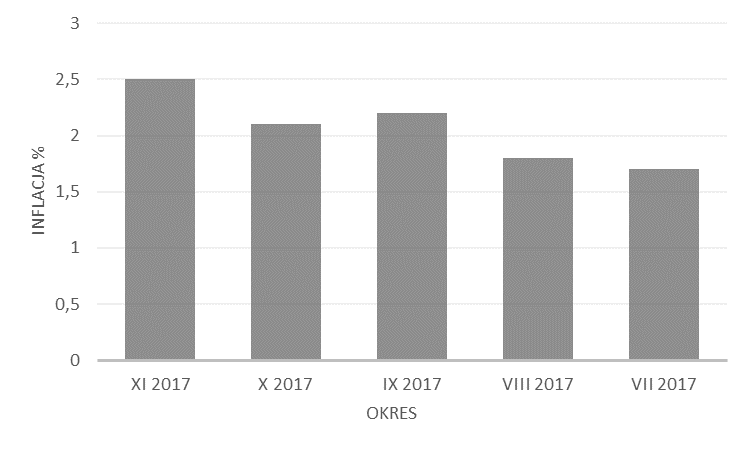
\includegraphics[width=150mm]{images/inflacja.png}
	\captionsource{Inflacja w Polsce.}{opracowanie własne.}
	\label{fig:inflacja}
\end{figure}

Na końcu pracy należy umieścić wykaz (spis) występujących w pracy rysunków uporządkowany wg kolejności ich występowania w dokumencie.



\section{Tabele}

Należy zwrócić szczególną uwagę na redagowanie tabel. Każda tabela powinna posiadać tytuł, kolejny numer oraz źródło pochodzenia danych. Tabelę należy wyśrodkować na stronie dokumentu. Jeśli to możliwe, powinno unikać się dzielenia tabel i umieszczać je w całości na jednej stronie. Do każdej tabeli należy umieścić odniesienie w tekście pracy zawierające jej numer. Pierwsze odwołanie musi wystąpić przed pojawieniem się tabeli w dokumencie, przy czym tabela nie musi występować bezpośrednio po tym odwołaniu, np. na tej samej stronie, np.

(...) z danych przedstawionych w tabeli \ref{tab:inflacja} wynika, iż w Polsce zaobserwować można powolny wzrost inflacji począwszy od drugiego półrocza 2017 roku (...)

\begin{table}[ht]
	\captionsource{Inflacja w Polsce.}{opracowanie własne.}
	\label{tab:inflacja}
	\centering
	\begin{tabular}{ l c }
		\hline
		\textbf{Okres}  &  \textbf{Wartość} \\ \hline
		XI 2017         &  2,5 \\
		X 2017          &  2,1 \\
		IX 2017         &  2,2 \\
		VIII 2017       &  1,8 \\
		VII 2017        &  1,7 \\ \hline
	\end{tabular}
	
\end{table}

 Wszystkie tabele występujące pracy powinny zostać sformatowanie w jednolity sposób i wyśrodkowane. Tytuł tabeli należy umieścić nad tabelą, a do jego formatowania wykorzystać styl Tytuł tabeli. Pod tabelą należy bezwzględnie podać źródło pochodzenia tabeli. Paragraf ten należy sformatować przy użyciu stylu Źródło.


Na końcu pracy należy umieścić wykaz (spis) występujących w pracy tabel uporządkowany wg kolejności ich występowania w dokumencie.



\section{Wzory}

Tu przykłady stosowania wzorów, np.

\begin{equation}
a^x+y \neq a^{x+y}
\end{equation}





